\documentclass[runningheads]{llncs}
\usepackage{graphicx}
\usepackage{url}
\usepackage{listings}
\usepackage{lstautogobble}
\graphicspath{ {./images/} }


\begin{document}

\lstset{
    language=prolog,
    autogobble=true,
    numbers=left
}

\title{Game Development with Answer Set Programming}
\subtitle{DaBlocksWorld}
\author{Dario Klepoch}
\authorrunning{Dario Klepoch}
\institute{Potsdam University}
\maketitle        

    \begin{abstract}
        Answer set programming (ASP) is declarative programming paradigm in which a problem is modeled through prolog-like rules.
        The idea is to represent a problem by a logic program where terms of rules will be used to formulate the constraints of the problem.
        Clingo contains a state-of-the-art grounder and solver for ASP encodings
        which here will be utilized to solve the `Blocks World' planning problem.
        Clingo will be combined with the open source Game engine `Godot' to generate random blocks world instances and solve them.
    \end{abstract}


    \section{Introduction}
        This paper aims to give an introduction to the `blocks world' planning problem and how to find optimal solutions for this problem.
        We will be developing an interactive game around this problem and show how Answer Set Programming (ASP) can
        be used to solve arbitrary configurations.\newline
        The blocks world planning problem consists of blocks which need to be move to certain positions.
        Those blocks can either be placed on a table or be stacked onto each other.
        In our game we will first generate a random block configuration.
        This random configuration will be parsed into facts which will be the input for Clingo (a combination of an ASP solver and grounder).
        Afterwards we will use the output of Clingo to rate the player's performance of solving the puzzle.\newline
        The first section of this paper will try to explain the Blocks World planning problem (BWPP) in a detailed way.
        The following section will explain the modifications we made to the BWPP and why we made them.
        The third section will be targeted towards the Godot game engine we used to implement the interactive part of this project.
        Finally we want to talk about the algorithm which generates and solves BWPP configurations.

    \section{The Blocks World planning problem}
        The BWPP is a planning problem in which blocks need to be restacked onto each other.
        Multiple blocks on top of each other are called a stack.
        The ground is the lowest point where a block can be placed.
        A stack is always rooted on the ground.
        This means that the lowest block of the stack is always on the ground.
        To this extend it is similar to the `towers of hanoi'-problem.
        However the blocks are all uniquely identifiable by numbers.
        An example of the BWPP is shown in figure \ref{startConfiguration}

        \begin{figure}[h]
            \centering
            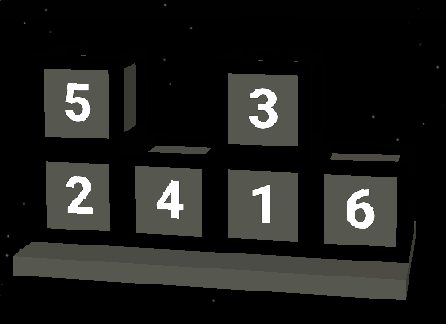
\includegraphics[width=6cm]{start_config.png}
            \caption{An example start configuration}
            \label{startConfiguration}
        \end{figure}

        But the order in which those stacks are placed on the table does not matter.
        This leads to the existence of ambiguous blocks world configurations.
        Figure \ref{ambiguousGoalConfig} shows two different looking configurations.
        However they are the same configuration in regards to the BWPP because only the placement of the stacks is different.
        
        \begin{figure}[h]
            \centering
            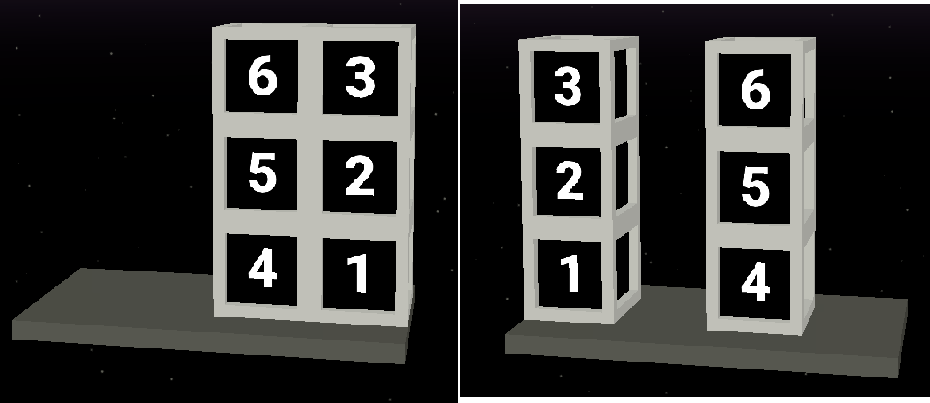
\includegraphics[width=8cm]{ambiguous_goal_config.png}
            \caption{Ambiguous goal configurations}
            \label{ambiguousGoalConfig}
        \end{figure}

        For each blocks world exists a start configuration and a goal configuration.
        The puzzle begins in the start configuration and should be transformed into the goal configuration only using legal moves.
        Legal moves are moves which correspond to the following rules:
        \begin{itemize}
            \item at one time step only one move can be executed 
            \item a block can only be moved if it has no other blocks on top
            \item a block can always be moved to the table to create a new stack
        \end{itemize}
        Now the challenge is to find the shortest series of legal moves to convert the start configuration into the goal configuration.\newline
        Figure \ref{goalOfTheBWPP} shows the goal of the BWPP.
        On the left hand side is the start configuration shown and on the right hand side is the goal configuration shown.
        \begin{figure}
            \centering
            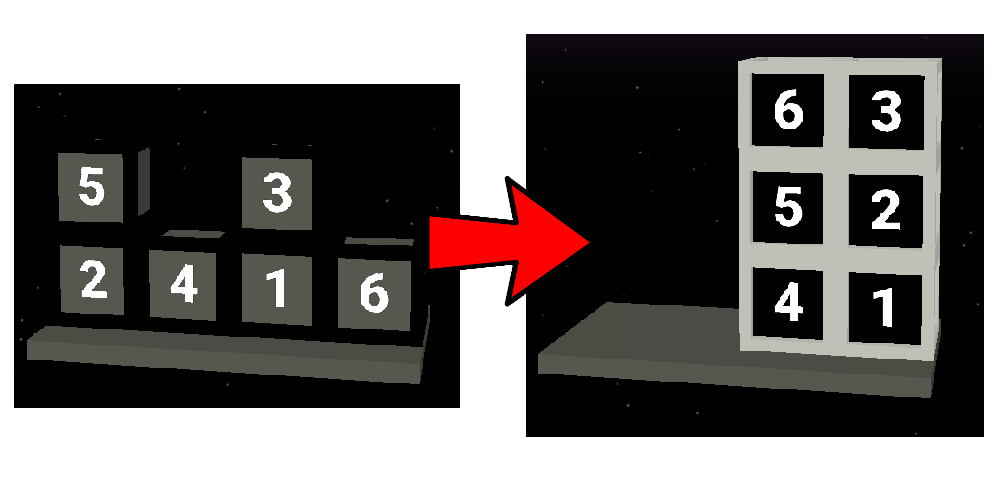
\includegraphics[width=9cm]{start_goal_config.png}
            \caption{Goal of the BWPP}
            \label{goalOfTheBWPP}
        \end{figure}

    \section{Godot}
        Godot is a completely free and open source game engine.
        It provides many tools for game development and design.
        Because it falls under the very permissive MIT license like Clingo 
        they are a perfect match for commercial game as no royalty fees will be charged.
        Godot is written in C/C++ and has designed its own scripting language: GodotScript (GDScript) \cite{godotWebsite}.
        But there is also a version of the game engine which enables the possibility to develop using C\#.
        This means one can develop in the Godot game engine using C/C++/C\#/GDScript.
        Because the benefit of a higher performance when using C/C++/C\# \cite{godotPerformanceComparison} is negligible in this project,
        GDScript was used.\newline
        In the current implementation of this project the ready made versions of Clingo for OSX, Windows and Linux \cite{clingoGithub} were used.
        This however limits our target platform to these three.
        Godot provides an interface called GDNative.
        This makes it possible to use custom C++ code in your game.
        Therefore it should be possible to use the source code of Clingo \cite{clingoGithub} and reach more platforms like android, iOS  
        
    \section{Game design decisions}
        Because this projects aims to provide a somewhat enjoyable gaming experience the standard BWPP got modified.
        The modifications aim to make the game understandable with only a few explanations.
        Ideally somebody who does not know the BWPP understands the game without further explanation.
        For better differentiation this project got the name `DaBlocksWorld'.\newline
        The first modification was that the maximum number of blocks which can be stacked onto each other got limited.
        This was necessary as the screen on which the game would be played is obviously limited in size.
        For the same reason the maximum number of stacks which can be placed on the table got limited too.\newline
        The next modification is due to the fact that the order of the block-stacks does not matter as shown in \ref{ambiguousGoalConfig}.
        Therefore the blocks were not labeled with subsequent numbers starting by $1$ till $ numberOfBlocks$,
        rather with numbers from 1 to $ numberOfBlocks / numberOfStacks$.
        This modification was made with the intention to show that the placement of the stacks is unimportant.
        This however leads to the problem that one does not know which of the multiple numbers needs to be placed on which stack.
        As an example: if there are 3 stacks from 1 to 3 it is not clear which 2 needs to be placed on which 1.
        To overcome this problem the blocks which belong to the same stack got the same color.
        The modifications can been seen in figure \ref{colorizedGoal}.
        On the left side the new start configuration can be seen and ob the right side the new goal configuration.\newline
        
        \begin{figure}[h]
            \centering
            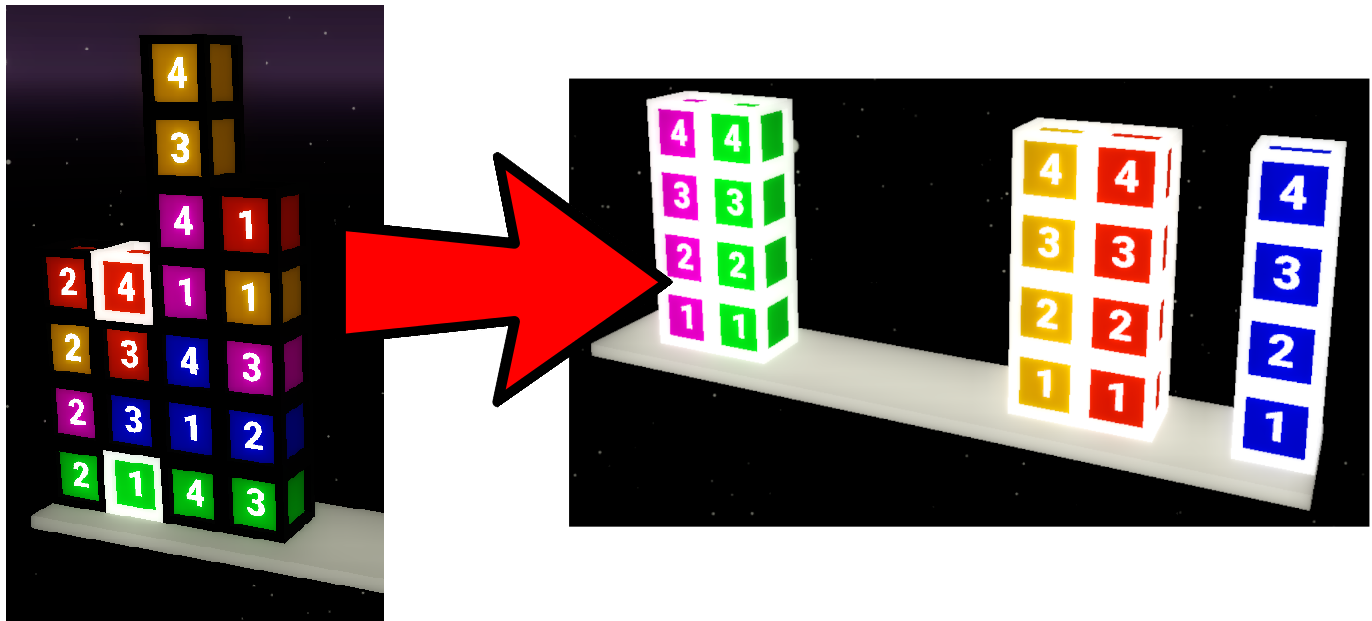
\includegraphics[width=10cm]{start_goal_config_colored.png}
            \caption{Changed BWPP and goal}
            \label{colorizedGoal}
        \end{figure}
        
        Additionally the player can decide a level of difficulty he or she wants to play.
        This difficulty changes the amount of blocks which will be given in the puzzle.
        And also set the maximum bounds for the puzzle.
        This means that the amount of stacks which can be placed on the board and also the height of those stacks change with the selected difficulty.

    \section{Generating and solving configurations}
        In the custom scripting language GodotScript a generator for BWPP configurations got developed.
        The main logical part of this generator can be found in listing \ref{generatingConfiguration}.
        How the graphics work will be excluded entirely from this paper because it would go beyond the scope of it. \newline
        `self.numOfBlocks' tells the game how many blocks should be placed in the current puzzle. 
        Now the generator creates a block according to this number (line 2).
        `generateRandomBlock()' returns a random Vector3 which is always inside of the bounds given by the selected difficulty.
        And also is not on the same position as a block which got instantiated earlier.\newline
        The last part of the generator applies `gravity' to the block.
        This simply pushes the block down until it either hits another block or the ground.

        \begin{lstlisting}[caption=Generating configuration, label=generatingConfiguration, language=python]
            func generateStartBoard():   
                for b in range(self.numOfBlocks):
                    ... 
                    #create random block coordinate for the currentBoard
                    var rndBlockCur = generateRandomBlock() 
                    ...
                    rndBlockCur.applyGravity()


            func generateRandomBlock() -> Vector3:
                var randX : int
                var randY : int
                var valid : bool = false

                while !valid:
                    randX = randi() % self.maxGenLength
                    randY = randi() % self.maxGenHeight
                    
                    #make sure there is no block on this cell
                    if(board[randX][randY] == 0):
                        valid = true

                return Vector3(randX, randY, 0)
        \end{lstlisting}
           
        In \cite{originalEncodingPaper} a solver for arbitrary BWPP configurations got developed.
        For this project the encoding from this paper was used as a baseline and got extended to suit the modified problem.
        In listing \ref{modification} one can see the modifications which where made to the base encoding.\newline
        $blocksOnGround(A, t)$ simply keeps track of the amount of blocks $A$ which are on the ground at a specific point in time $t$.
        $height(B, H, t)$ counts for every block $B$ the height $H$ at the point in time $t$ by recursively adding the blocks up.

        \begin{lstlisting}[caption=Addition to the encoding, label=modification]
            %DEFINE
            ...
            blocksOnGround(A, t) :- #count{X : on(X, 0, t)} = A.
            height(B, 1, t) :- on(B, 0, t).
            height(B1, H+1, t) :- height(B2, H, t), on(B1, B2, t),
                                amountOfBlocks(A), H < A.
        \end{lstlisting}
        
        Finally the board gets resized.
        The size is exactly the size that the optimal plan found by clingo can be executed by the player.
        The height is the highest $H$ of all $height/3$ and the length is the highest $A$ of all $blocksOnGround/2$.

    \section{Conclusion}
        With DaBlocksWorld \cite{daBlocksWorldGithub} a game was developed only using open source tools and software.
        In the scripting language of Godot: `GDScript' a random generator for `Block World' puzzles was written.
        Using the Answer Set Programing paradigm a solver for every possible generated puzzle got utilized to solve this generated puzzle.
        While the player is solving the game he can always see the minimum numbers of moves necessary to solve this puzzle and also his own number of moves.
        The game and source of this project is available from \cite{daBlocksWorldGithub}.\newline
        With the power of an effective ASP solver and grounder new possibilities in the space of Game Design are possible. 


    \begin{thebibliography}{8}

        \bibitem{godotWebsite}
            \url{https://godotengine.org/},
            last access: 12.3.2020

        \bibitem{originalEncodingPaper}
            Modeling and Language Extensions,
            \url{https://aaai.org/ojs/index.php/aimagazine/article/view/2673},
            author: Torsten Schaub, Martin Gebser,
            last access: 14.3.2020

        \bibitem{cApi}
            \url{https://docs.godotengine.org/en/3.1/tutorials/plugins/gdnative/gdnative-cpp-example.html},
            last access: 13.3.2020

        \bibitem{gdNativeExample}
            \url{https://docs.godotengine.org/en/3.2/tutorials/plugins/gdnative/gdnative-c-example.html},
            last access: 13.3.2020

        \bibitem{daBlocksWorldGithub}
            \url{https://github.com/CaptainDario/DaBlocksWorld}

        \bibitem{godotPerformanceComparison}
            \url{https://github.com/cart/godot3-bunnymark#user-content-benchmark-run---february-22-2018},
            last access: 12.3.2020

        \bibitem{clingoGithub}
            \url{https://github.com/potassco/clingo},
            last access: 10.3.2020

    \end{thebibliography}
\end{document}